\documentclass[12pt]{article}
\usepackage[utf8]{inputenc}
\usepackage[automark]{scrlayer-scrpage}
\usepackage[T1]{fontenc}
\usepackage[pdftex]{graphicx,color}
\usepackage{subcaption}
\usepackage{url}
\usepackage[pdftex,pdfpagelabels]{hyperref}
\usepackage[section,boxed]{algorithm}
\usepackage{algpseudocode}
\usepackage{amsmath}
\usepackage{amssymb}
\usepackage{amsthm}
\usepackage{lmodern}
\pagestyle{scrheadings}
\ofoot{}\cfoot{}\ifoot{}
\lehead{\pagemark}
\rehead{\slshape\leftmark}
\lohead{\slshape\leftmark}
\rohead{\pagemark}
\newtheorem{definition}{Definition}
\newtheorem{theorem}{Theorem}
\usepackage{blindtext}
\usepackage[ngerman]{babel}
\usepackage[margin=1in]{geometry}
\usepackage{amsmath,amsthm,amssymb}
\usepackage{graphicx}
\newcommand{\N}{\mathbb{N}}
\newcommand{\Z}{\mathbb{Z}}
\newcommand{\R}{\mathbb{R}}
\newcommand{\C}{\mathbb{C}}

\begin{document}
% --------------------------------------------------------------
%                         Title Page
% --------------------------------------------------------------
\title{Solutions for Sheet 5}
\author{Raphael Wude, Martin Brückmann, Claude Jordan, Daniel Degenstein\\ \\
\textsc{Pattern Matching and Machine Learning} \\
\textsc{for Audio Signal Processing}}
\maketitle

% --------------------------------------------------------------
%                         Task 1.1
% --------------------------------------------------------------
\section*{Task 5.1}
\begin{itemize}
    \item[(a)]
    Let $x=[3,1,0,0,2]$ be a vector. The cyclic autocorrelation of the vector is:
    \begin{align*}
        ACF[x](0) &= \langle x | T_0(x) \rangle \\
        &= \langle [3,1,0,0,2] ~|~ [3,1,0,0,2] \rangle = 13\\
        ACF[x](1) &= \langle x | T_1(x) \rangle \\
        &= \langle [3,1,0,0,2] ~|~ [2,3,1,0,0] \rangle = 9\\
         ACF[x](2) &= \langle x | T_2(x) \rangle \\
        &= \langle [3,1,0,0,2] ~|~ [0,2,3,1,0] \rangle = 2\\
        ACF[x](3) &= \langle x | T_3(x) \rangle \\
        &= \langle [3,1,0,0,2] ~|~ [0,0,2,3,1] \rangle = 2\\
        ACF[x](4) &= \langle x | T_4(x) \rangle \\
        &= \langle [3,1,0,0,2] ~|~ [1,0,0,2,3] \rangle = 9\\
    \end{align*}

    \item[b)]
    Let $x = [3,1,0,0,2]$ and $y=[1,3,2,0,1]$ be two vectors. The cyclic convolution of the vectors is:
    \begin{align*}
        (x*y)(0) &= \sum_{n=0}^{N-1}x(n) \cdot y(-n \text{ mod } N)\\
        &= 3 \cdot y(0) + 1 \cdot y(4) + 0 \cdot y(3) + 0 \cdot y(2) + 2 \cdot y(1) = 3 + 1 + 6 = 10\\
        (x*y)(1) &= \sum_{n=0}^{N-1}x(n) \cdot y(1-n \text{ mod } N)\\
        &= 3 \cdot y(1) + 1 \cdot y(0) + 0 \cdot y(4) + 0 \cdot y(3) + 2 \cdot y(2) = 9 + 1 + 4 = 14\\
        (x*y)(2) &= \sum_{n=0}^{N-1}x(n) \cdot y(2-n \text{ mod } N)\\
        &= 3 \cdot y(2) + 1 \cdot y(1) + 0 \cdot y(0) + 0 \cdot y(4) + 2 \cdot y(3) = 6 + 3 = 9\\
        (x*y)(3) &= \sum_{n=0}^{N-1}x(n) \cdot y(3-n \text{ mod } N)\\
        &= 3 \cdot y(3) + 1 \cdot y(2) + 0 \cdot y(1) + 0 \cdot y(0) + 2 \cdot y(4) = 2 + 2 = 4\\
        (x*y)(4) &= \sum_{n=0}^{N-1}x(n) \cdot y(4-n \text{ mod } N)\\
        &= 3 \cdot y(4) + 1 \cdot y(3) + 0 \cdot y(2) + 0 \cdot y(1) + 2 \cdot y(0) = 3 + 2 = 5
    \end{align*}
    \item[c) \& d)]
    \begin{figure}[h]
        \centering
        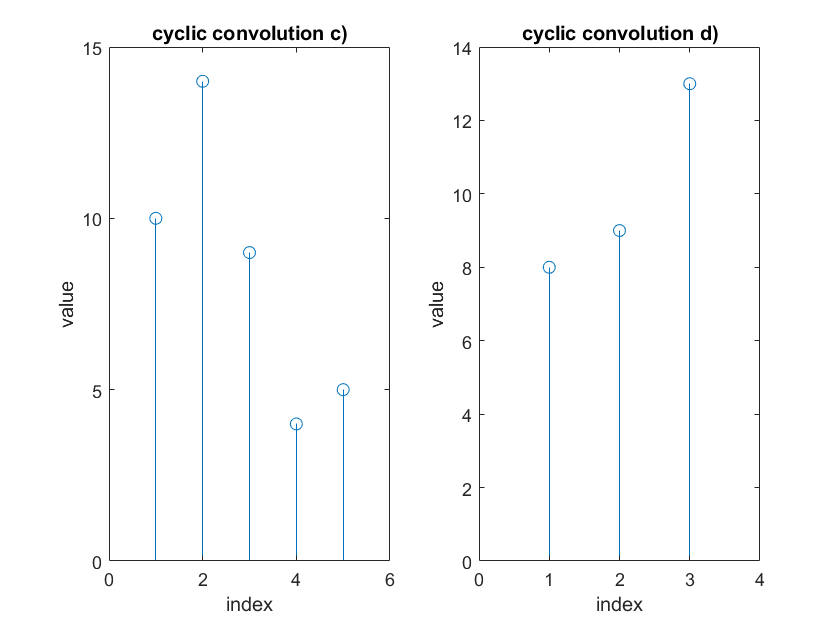
\includegraphics[width=1.1\textwidth]{Sheet05Exercise1.png}
    \end{figure}
\end{itemize}
\newpage

\section*{Task 5.2}
The frequency response $H(\omega)$ of

\[
h(\omega) =
    \begin{cases}
        \frac{1}{3} & \quad\text{if } n=0,1,2\\
        0 &\quad\text{else.}
    \end{cases}
\]

is given by

\begin{align*}
    H(\omega) :&= \sum_{k \in \mathbb{Z}} h(k)e^{-2 \pi i \omega k}\\
    &= h(0) \cdot e^{-2 \pi i \omega \cdot 0} + h(1) \cdot e^{-2 \pi i \omega \cdot 1} + h(2) \cdot e^{-2 \pi i \omega \cdot 2}\\
    &= \frac{1}{3} (1 + e^{-2 \pi i \omega} + e^{-4 \pi i \omega})
\end{align*}

\section*{Task 5.3}

\subsection*{(a)}
Write $h$ as a vector:
\[
\begin{pmatrix}
h(k_{1})\\
h(k_{2})\\
\vdots\\
h(k_{n})
\end{pmatrix}
\]
Now write $x$ as a matrix:
\[
\begin{pmatrix}
x(1-k_{1}) & x(1-k_{2}) & \cdots & x(1-k_{n})\\
x(2-k_{1}) & x(2-k_{2}) & \cdots & x(2-k_{n})\\
\vdots & \vdots & \ddots & \vdots\\
x(n-k_{1}) & x(n-k_{2}) & \cdots & x(n-k_{n})
\end{pmatrix}
\]
\\\\Now we can write $C_{h}[x]$ as a matrix $\times$ vector product:
\[
\begin{pmatrix}
x(1-k_{1}) & x(1-k_{2}) & \cdots & x(1-k_{n})\\
x(2-k_{1}) & x(2-k_{2}) & \cdots & x(2-k_{n})\\
\vdots & \vdots & \ddots & \vdots\\
x(n-k_{1}) & x(n-k_{2}) & \cdots & x(n-k_{n})
\end{pmatrix} \times \begin{pmatrix}
h(k_{1})\\
h(k_{2})\\
\vdots\\
h(k_{n})
\end{pmatrix}
\]
\[
~~~~~~~~~~~= \begin{pmatrix}
x(1-k_{1}) \cdot h(k_{1}) + x(1-k_{2}) \cdot h(k_{2}) + \ldots + x(1-k_{n}) \cdot h(k_{n})\\
x(2-k_{1}) \cdot h(k_{1}) + x(2-k_{2}) \cdot h(k_{2}) + \ldots + x(2-k_{n}) \cdot h(k_{n})\\
\vdots\\
x(n-k_{1}) \cdot h(k_{1}) + x(n-k_{2}) \cdot h(k_{2}) + \ldots + x(n-k_{n}) \cdot h(k_{n})
\end{pmatrix}
\]
\[
= \begin{pmatrix}
(h*x)(1)\\
(h*x)(2)\\
\vdots\\
(h*x)(n)
\end{pmatrix}~~~~~~~~~~~~~~~~~~~~~~~~~~~~~~~~~~~~~~~~~~~~~~~~~~~~~~~
\]

\subsection*{(b)}

\end{document}
